\documentclass[a4paper, man, floatsintext]{apa6}
\usepackage{lmodern}
\usepackage{amssymb,amsmath}
\usepackage{ifxetex,ifluatex}
\usepackage{fixltx2e} % provides \textsubscript
\ifnum 0\ifxetex 1\fi\ifluatex 1\fi=0 % if pdftex
  \usepackage[T1]{fontenc}
  \usepackage[utf8]{inputenc}
\else % if luatex or xelatex
  \ifxetex
    \usepackage{mathspec}
  \else
    \usepackage{fontspec}
  \fi
  \defaultfontfeatures{Ligatures=TeX,Scale=MatchLowercase}
\fi
% use upquote if available, for straight quotes in verbatim environments
\IfFileExists{upquote.sty}{\usepackage{upquote}}{}
% use microtype if available
\IfFileExists{microtype.sty}{%
\usepackage{microtype}
\UseMicrotypeSet[protrusion]{basicmath} % disable protrusion for tt fonts
}{}
\usepackage{hyperref}
\hypersetup{unicode=true,
            pdfauthor={Jana B. Jarecki},
            pdfborder={0 0 0},
            breaklinks=true}
\urlstyle{same}  % don't use monospace font for urls
\usepackage{graphicx,grffile}
\makeatletter
\def\maxwidth{\ifdim\Gin@nat@width>\linewidth\linewidth\else\Gin@nat@width\fi}
\def\maxheight{\ifdim\Gin@nat@height>\textheight\textheight\else\Gin@nat@height\fi}
\makeatother
% Scale images if necessary, so that they will not overflow the page
% margins by default, and it is still possible to overwrite the defaults
% using explicit options in \includegraphics[width, height, ...]{}
\setkeys{Gin}{width=\maxwidth,height=\maxheight,keepaspectratio}
\IfFileExists{parskip.sty}{%
\usepackage{parskip}
}{% else
\setlength{\parindent}{0pt}
\setlength{\parskip}{6pt plus 2pt minus 1pt}
}
\setlength{\emergencystretch}{3em}  % prevent overfull lines
\providecommand{\tightlist}{%
  \setlength{\itemsep}{0pt}\setlength{\parskip}{0pt}}
\setcounter{secnumdepth}{0}
% Redefines (sub)paragraphs to behave more like sections
\ifx\paragraph\undefined\else
\let\oldparagraph\paragraph
\renewcommand{\paragraph}[1]{\oldparagraph{#1}\mbox{}}
\fi
\ifx\subparagraph\undefined\else
\let\oldsubparagraph\subparagraph
\renewcommand{\subparagraph}[1]{\oldsubparagraph{#1}\mbox{}}
\fi

%%% Use protect on footnotes to avoid problems with footnotes in titles
\let\rmarkdownfootnote\footnote%
\def\footnote{\protect\rmarkdownfootnote}

%%% Change title format to be more compact
\usepackage{titling}

% Create subtitle command for use in maketitle
\providecommand{\subtitle}[1]{
  \posttitle{
    \begin{center}\large#1\end{center}
    }
}

\setlength{\droptitle}{-2em}

  \title{}
    \pretitle{\vspace{\droptitle}}
  \posttitle{}
    \author{Jana B. Jarecki}
    \preauthor{\centering\large\emph}
  \postauthor{\par}
      \predate{\centering\large\emph}
  \postdate{\par}
    \date{17 September, 2019}

\usepackage{natbib} \usepackage{threeparttable} \usepackage{booktabs}
\shorttitle{test} \usepackage{setspace}
\AtBeginEnvironment{tabular}{\singlespacing} \usepackage{times}
\usepackage{changes} \definechangesauthor[name={JJ}, color=orange]{jj}
\usepackage{upgreek} \AtBeginDocument{\let\maketitle\relax}

\begin{document}

\subsection{Evaluations of Gambles by Condition and Sample Size}

Table \ref{tab:means_study1} shows participants' evaluations of the
gambles in the experience and description conditions. Notably, the
evaluations in the experience condition stay relatively constant across
sample sizes. In the best-fitting mixed regression model
\(\mathrm{M}\textsubscript{0}\) sample size was included as a random
effect, and gamble type---p-bet vs. \$-bet---as a fixed effect,
resulting in higher evaluations of the p-bets (gamble IDs 1 to 3)
compared to the \$-bets (IDs 4 to 6). This model outperformed a model
with sample size as fixed effect (\(BF\textsubscript{01} = 409\)), and a
model with a sample-size\(\times\)gamble-type interaction
(\(BF\textsubscript{01} > 1,000\)).

\begin{table}[tbp]
\begin{center}
\begin{threeparttable}
\caption{\label{tab:means_study1}Valuations of Gambles in Study 1}
\begin{tabular}{lcccrr}
\toprule
Condition & Sample size & \textit{Med} & \textit{M} & D--E & D--E:$BF\textsubscript{10}$\\
\midrule
Gamble ID 1 &  &  &  &  & \\
\ \ \ E & xs & 5.00 & 5.16 & -0.56 & NA\\
\ \ \ E & s & 4.55 & 5.30 & -0.70 & NA\\
\ \ \ E & m & 5.00 & 5.34 & -0.74 & NA\\
\ \ \ E & l & 5.00 & 5.29 & -0.69 & NA\\
\ \ \ D & NA & 4.00 & 4.60 & NA & NA\\
Gamble ID 2 &  &  &  &  & \\
\ \ \ E & xs & 4.00 & 4.33 & -0.71 & NA\\
\ \ \ E & s & 4.00 & 4.31 & -0.69 & NA\\
\ \ \ E & m & 4.00 & 4.04 & -0.43 & NA\\
\ \ \ E & l & 4.00 & 3.99 & -0.37 & NA\\
\ \ \ D & NA & 3.00 & 3.61 & NA & NA\\
Gamble ID 3 &  &  &  &  & \\
\ \ \ E & xs & 6.00 & 7.56 & -0.99 & NA\\
\ \ \ E & s & 6.70 & 8.40 & -1.83 & NA\\
\ \ \ E & m & 6.20 & 7.92 & -1.35 & NA\\
\ \ \ E & l & 6.00 & 7.68 & -1.11 & NA\\
\ \ \ D & NA & 5.00 & 6.57 & NA & NA\\
Gamble ID 4 &  &  &  &  & \\
\ \ \ E & xs & 3.00 & 2.80 & 0.28 & NA\\
\ \ \ E & s & 3.20 & 2.91 & 0.16 & NA\\
\ \ \ E & m & 3.00 & 2.80 & 0.28 & NA\\
\ \ \ E & l & 3.00 & 2.95 & 0.13 & NA\\
\ \ \ D & NA & 3.20 & 3.08 & NA & NA\\
Gamble ID 5 &  &  &  &  & \\
\ \ \ E & xs & 2.00 & 1.77 & 0.10 & NA\\
\ \ \ E & s & 2.00 & 1.75 & 0.12 & NA\\
\ \ \ E & m & 2.00 & 1.73 & 0.14 & NA\\
\ \ \ E & l & 2.00 & 1.81 & 0.06 & NA\\
\ \ \ D & NA & 2.00 & 1.87 & NA & NA\\
Gamble ID 6 &  &  &  &  & \\
\ \ \ E & xs & 4.00 & 3.46 & 0.18 & NA\\
\ \ \ E & s & 4.00 & 3.55 & 0.09 & NA\\
\ \ \ E & m & 4.00 & 3.58 & 0.06 & NA\\
\ \ \ E & l & 4.00 & 3.70 & -0.06 & NA\\
\ \ \ D & NA & 4.00 & 3.64 & NA & NA\\
\bottomrule
\addlinespace
\end{tabular}
\begin{tablenotes}[para]
\normalsize{\textit{Note.} \textit{M} = mean, \textit{Med} = median, D--E = difference between mean description-based valuations and experience-based valuations, $BF\textsubscript{10}$ = Bayes Factor quantifying the evidence for a linear model $\mathrm{M}\textsubscript{1}$ predicting that valuations differ between description and experience over a linear model $\mathrm{M}\textsubscript{0}$ predicting no such differences; both models models contain a by-participant random effect. Gambles IDs 1, 2, and 3 are \$-bets; Gamble IDs 4, 5, and 6 are p-bets.}
\end{tablenotes}
\end{threeparttable}
\end{center}
\end{table}

\subsection{Cognitive Modeling of Experience-based Evaluations by Sample Size}

To unpack the role of sample size in value judgments more closely, we
used cognitive computational modeling. We compared the performance of
the \added[id=jj]{relative frequency} (RF) model and the
\added[id=jj]{Bayesian value updating} (BVU) model regarding the
observed evaluations.
\added{The models were compared to a baseline model, predicting a constant evaluation equal to the mean  individual evaluation (sensible models are expected to outperform this baseline model).}

\subsubsection{Modeling Procedure}

\added[id=jj]{The observed and predicted evaluations were normalized to a common range (0 - 1, by division through the gain magnitude and truncation of normalized values $>$ 1). The free model parameters were estimated by maximum likelihood at the participant level, assuming observations follow a truncated normal distribution, censored at 0 and 1, around the model predictions with a constant standard deviation ($\sigma$) estimated as a free parameter ($0 < \sigma \leq 1$).  Therefore, the relative frequency model had 2 free parameter, the power utility exponent $\alpha$ ($0 \leq \alpha \leq 20$) and $\sigma$. The Bayesian value updating model had 4 free parameter the gain prior $\theta_G$ ($0 \leq \theta_G \leq 1$; the loss prior was $\theta_0=2-\theta_G$), the learning rate $\delta$ ($0 \leq \delta \leq 10$), $\alpha$ and $\sigma$. A 3-parameter Bayesian value updating model was also tested, which had a fixed learning rate of $\delta=1$ (optimal Bayesian updating). The baseline model had 2 free parameter, the mean evaluation $\mu$ and $\sigma$. We estimated the parameters with a local solver using a augmented Lagrange multiplier method \citep[Rsolnp package, version 1.16]{Ghalanos2015}. We compared the models by the Bayesian information criterion (BIC), transformed into Bayesian evidence weights \citep[][1 means very strong evidence for a competitor model]{Kass1995, Lewandowsky2011}}.

\subsubsection{Modeling Results}
\added[id=jj]{We will first outline the quantitative model fit, followed by the qualitative model fit, and lastly analyze the effects of sample size given the cognitive strategies.}
\subsubsection{Quantitative Model Fit.}

The Bayesian value updating model described about half of the
participants best (22 of 40; 55\%), and the relative frequency model
described a minority of participants (13; 32\%). The baseline model
described 5 participants best. Figure \ref{fig:model_weights} shows the
evidence strength for the models by participant. It becomes evident that
the 3-parameter BVU competes mostly with the full BVU model. The mean
Bayesian information criterion (BIC) across participants of the models
equaled BIC\textsubscript{BVU}\(=\) -109.5, BIC\textsubscript{RF}\(=\)
-109.1, and BIC\textsubscript{BASE}\(=\) -16.7.

\begin{figure}

{\centering 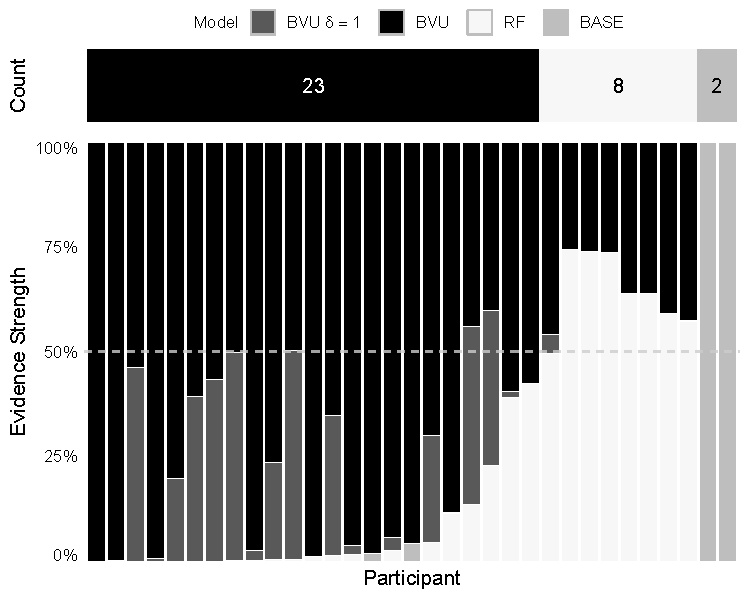
\includegraphics{../figures/model_weights-1} 

}

\caption{Evidence for the models for individual participants. \textit{RF}$=$ relative frequency model, \textit{BVU}$=$ Bayesian value updating model, \textit{BASE}$=$ Baseline model.}\label{fig:model_weights}
\end{figure}

The estimated parameter of the winning models, shown in Table
\ref{tab:model_par}, reveal that the power utility exponent (\(\alpha\))
is almost identical for those participants using a Bayesian value
updating strategy (\(M_{\alpha}= 1.41\)) and those using a relative
frequency strategy (\(M_{\alpha}=1.45\)) \(\Delta M = -0.04\), 95\% CI
\([-0.60\), \(0.51]\), \(t(32.40) = -0.16\), \(p = .872\). The resulting
parameters of the Bayesian model also indicate a prior belief in gains
being less likely (B\textsubscript{BVU,0}=0.365\%) than zero outcomes
(\(\theta_G = 0.73, \theta_0 = 1.27\) prior on gains and zeros,
respectively).

\begin{table}[tbp]
\begin{center}
\begin{threeparttable}
\caption{\label{tab:model_par}Parameter Estimates of Winning Models, \textit{M (SD)}}
\begin{tabular}{lcccc}
\toprule
Winning Model & $\alpha$ & $\theta_G$ & $\mu$ & $\sigma$\\
\midrule
BVU (\textit{n}$=$22) & 1.41 (1.07) & 0.73 (0.65) & - & 0.15 (0.08)\\
RF (\textit{n}$=$13) & 1.45 (0.54) & - & - & 0.11 (0.03)\\
BASE (\textit{n}$=$5) & - & - & 0.50 (0.03) & 0.19 (0.06)\\
\bottomrule
\addlinespace
\end{tabular}
\begin{tablenotes}[para]
\normalsize{\textit{Note.} \textit{BVU}$=$ Bayesian value updating model, \textit{RF}$=$ relative frequency model, \textit{BASE}$=$baseline model. Parameters denote: $\alpha=$ power utility exponent, $\theta_G$ gain prior, $\mu=$ mean evaluation, $\sigma$ standard deviation.}
\end{tablenotes}
\end{threeparttable}
\end{center}
\end{table}
\subsubsection{Qualitative Model Fit.}
\added[id==jj]{To see the qualitative fit between the models and the observed data, we plotted participants' evaluations against the model predictions from the respective participant's best-fitting model with optimized parameters. This allows to examine the qualitative model performance. Figure \ref{fig:ind_fits1} shows that the models generally capture the data well, but in some cases, even the best-fitting model fails to describe the data. Specifically, for participants number 1, 19, 24, and 38, for whom the winning model is the Bayesian updating (BVU) model, even the Bayesian model must be rejected because it mis-fits the data qualitatively.}

\begin{figure}

{\centering 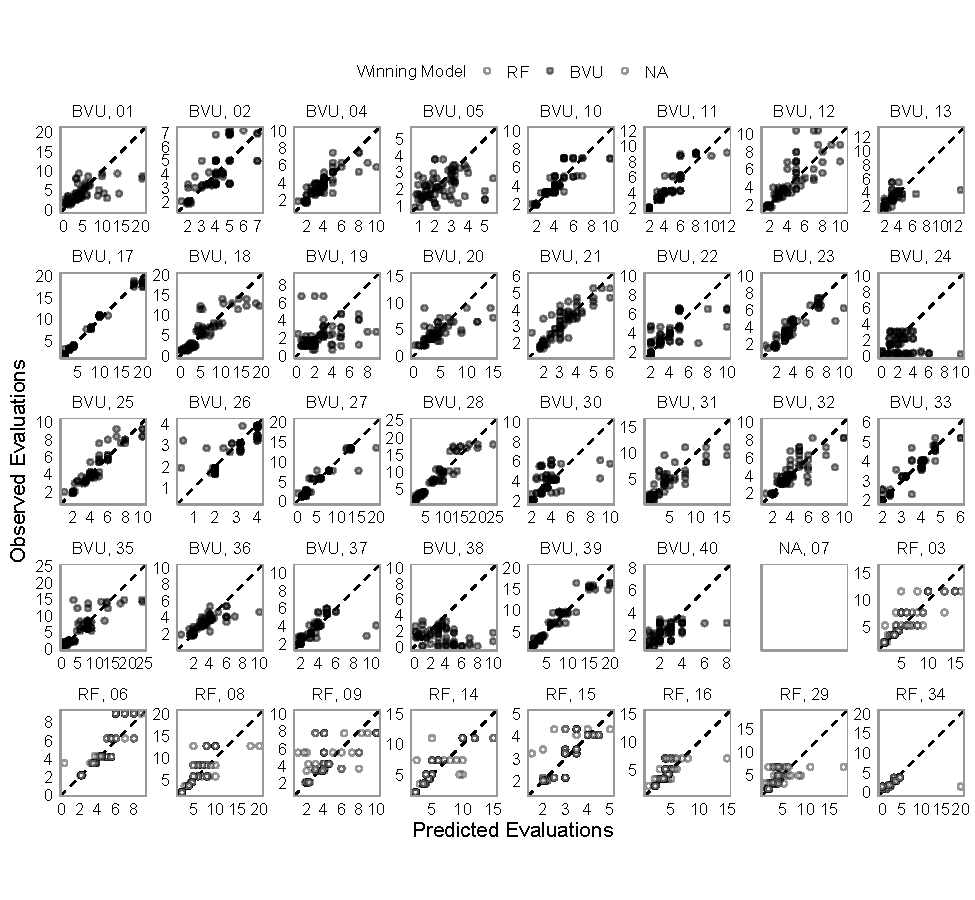
\includegraphics{../figures/ind_fits1-1} 

}

\caption{Predicted evaluations from the best-fitting models plotted against the observed evaluations (by participant). \textit{BVU}$=$ Bayesian value updating model, \textit{RF}$=$ relative frequency model, \textit{BASE}$=$baseline model.}\label{fig:ind_fits1}
\end{figure}

\added{Additionally, the cognitive modeling results help interpreting the null finding---that sample size has no effect on evaluations---that we observed at the aggregate level (Table \ref{tab:means_study1}). The aggregate analysis fails to take the heterogeneity in strategy use into account. The distribution of winning model indicates that our sample is best described by a mixture of strategies, which the aggregate analyses could not pick up. Moreover, the aggregate analysis fails to account for the prior beliefs regarding gain probabilities. Depending on the prior belief, the Bayesian value updating (BVU) model predicts either a decrease or an increase in valuations with increasing sample size.}

\emph{The effect of sample size given cognitive strategies.} Next, we
qualitatively analyzed if sample size differentially affects the
relative-frequency-type and Bayesian-type learners. We expected that
sample size changes evaluations of the Bayesian learners depending on
their priors, but that sample size does not change the evaluations of
the frequency-type learners.

\begin{figure}

{\centering 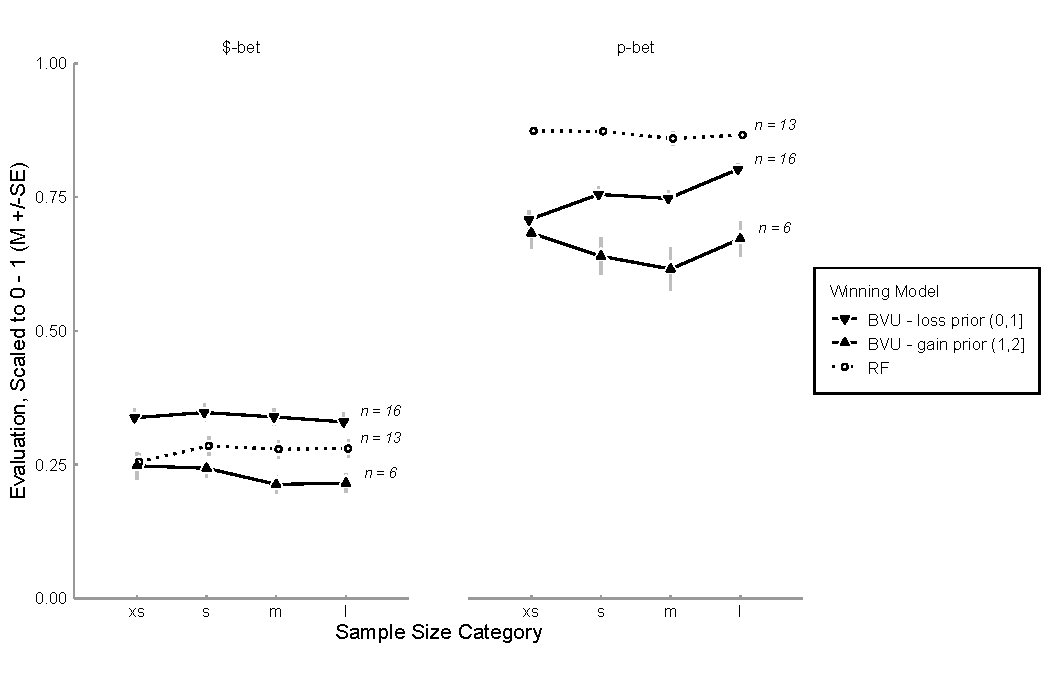
\includegraphics{../figures/qual1-1} 

}

\caption{Mean evaluation (standardized to 0 - 1) split by winning model and prior beliefs of the BVU model. \textit{BVU}$=$Bayesian value updating model, \textit{RF}$=$ Relative frequency model. Error bars indicate standard errors. \textit{\$-bet}: low-probability high-outcome gambles, \textit{p-bet}: high-probability low-outcome gambles. Sample sizes (xs, x, m, l), see Table \ref{tab:Lotteries}. \textit{N = 16, 13, 6} denotes the number of participants best-described by the respective models.}\label{fig:qual1}
\end{figure}

\added[id=jj]{
  To investigate the interaction of prior beliefs and sample size, we split the participants by cognitive strategy into three groups: relative frequency learners, Bayesian learners with a gain prior (prior parameter $\theta_G > 1$), and Bayesian learners with a loss prior (prior parameter $\theta_G \leq 1$). For relative-frequency learners we do not expect valuations to change with sample size; for the Bayesian learners with a high gain prior we expect valuations to decrease with sample size; for the Bayesian learners with a high zero-outcome prior, we expect valuations to increase with sample size. Figure \ref{fig:qual1} shows---separately for p-bets and \$-bets---how evaluations change for the three groups (relative frequency, Bayesian with gain prior, Bayesian with loss prior). The relative-frequency learners evaluated both p-bets and \$-bets relatively constantly across sample sizes, whereas the Bayesian learners increased their evaluations if they started with a loss prior and decreased their evaluations after starting with a gain prior, at least for p-bets (high-gain low-probability gambles). For \$-bets the Bayesian learners were relatively constant in their evaluations across sample sizes.
}


\end{document}
